\documentclass[a4paper,12pt]{article}
\usepackage[czech]{babel}
\usepackage[utf8]{inputenc}
\usepackage{graphicx}
\usepackage[absolute,overlay]{textpos} % Додає можливість абсолютного позиціонування

\begin{document}

% Титульна сторінка
\begin{titlepage}
    \centering
    \vspace*{\fill}
    {\LARGE \textbf{Ratatouille}}\\[0.3cm]
    Meal Organizer\\[1.5cm]
    Členové týmu:\\[0.5cm]
    Bilyk Vladyslava - kapitán \\
    \texttt{xbilyk03} \\[0.5cm]
    Kucher Maryna \\
    \texttt{xkuche01} 
    \vspace*{\fill}
\end{titlepage}

\newpage

\section*{Uživatelský průzkum a specifikace}

\subsection*{Popis aplikace}
    Moderní rytmus života nás nutí neustále hledat způsoby, jak efektivně hospodařit s časem a zdroji. Bez jasného plánu je obtížné kontrolovat výdaje: nakupujeme příliš mnoho, zapomínáme, co už máme, a utrácíme peníze za produkty, které se mohou zkazit, než je stihneme použít. Rozhodli jsme se vytvořit aplikaci, která pomáhá tyto problémy řešit. Usnadňuje uspořádání všech produktů, které již doma máte, plánování jídel na konkrétní dny, vytváření podrobných nákupních seznamů, sledování, kolik peněz utratíte za jídlo, a dokonce i kontrolu data expirace produktů. Tento přístup umožňuje nejen ušetřit čas a peníze, ale také diverzifikovat vaši menu.

\subsection*{Cílová skupina, pro kterou je program určen}
    Lidé, kteří si rádi organizují svůj život, věk: starší 16 let.
    


\subsection*{Požadavky uživatele}
\begin{itemize}
    \item Závěr z rozhovoru s uživatelem od Kucher Maryny
    \begin{itemize}
        \item Dotazovaný je osmnáctiletý člověk, který začal žít sám a rád využívá aplikace pro organizaci každodenních úkolů
        \item Uživatel potřebuje pohodlnou a srozumitelnou aplikaci, která mu pomůže organizovat zásoby jídla, plánovat jídelníček na několik dní dopředu a ušetřit čas při rozhodování, co vařit každý den.
        Uživatel by rád měl možnost automaticky sestavit menu na základě dostupných produktů a receptů, které si sám vybral. Chce mít možnost snadno přidávat nové položky, sledovat, co je skladem, a kontrolovat datum spotřeby produktů.
        Důležitou funkcí by měla být také možnost rychlého vytvoření nákupního seznamu podle plánovaných jídel nebo chybějících produktů. Uživatel by uvítal, kdyby aplikace dokázala zobrazit přibližné náklady na nákup a, ideálně, umožnila sledovat výdaje za určité období.
    \end{itemize}
    \item Závěr z rozhovoru s uživatelem od Bilyk Vladyslavy
    \begin{itemize}
        \item Byl proveden rozhovor s osobou, která pravidelně vaří pro celou rodinu a potřebuje pomocníka pro plánování jídel a nákupů potravin.
        \item Závěr z rozhovoru: Uživatel by si přál mít v programu rozvrh/kalendář jídel, aby měl před sebou plán, co bude třeba připravit na následující dny. V seznamu dostupných potravin by chtěl označit základní potraviny (jako je sůl, cukr, máslo, rýže atd.), a když by tyto potraviny došly, obdržet upozornění. Dále by ocenil upozornění, když nebudou k dispozici potraviny pro jídlo přidané do kalendáře. Zajímala by ho také funkce doporučení jídel, která je možné připravit z dostupných potravin. Z dalších přání: Uživatel by rád dostával upozornění z kalendáře před svátky a přidával do nákupního seznamu speciální produkty pro svátky, například alkohol nebo dort.
    \end{itemize}
    \item Závěr týmu
    \begin{itemize}
        \item Užvatelé chtějí aplikaci, která co nejvíce automatizuje plánování jídel a nákupní seznamy. uživatelé také projevili zájem o možnost sledovat další údaje o produktech, jako jsou data expirace nebo zvláštní pozornost při nákupu základních produktů.
    \end{itemize}
\end{itemize}

\section*{Průzkum existujících řešení}

\subsection*{Seznam aplikací. Pro a proti pro každou aplikaci}
\begin{itemize}
    \item \textbf{Mealime} : aplikace nabízí velkou databázi receptů s podrobným popisem vaření, možnost vytvoření nákupního seznamu.
    \begin{itemize}
        \item Výhoda :  Automatické vytváření nákupního seznamu. Možnost vařit s obrazem kroků receptu v reálném čase. Schopnost vytvářet si vlastní recepty nebo používat ty navržené.
        \item Nevyhoda : aplikace neposkytuje možnost ovládat seznam produktů, které jsou doma. Naplánované recepty nejsou propojeny s kalendářem.
    \end{itemize}
    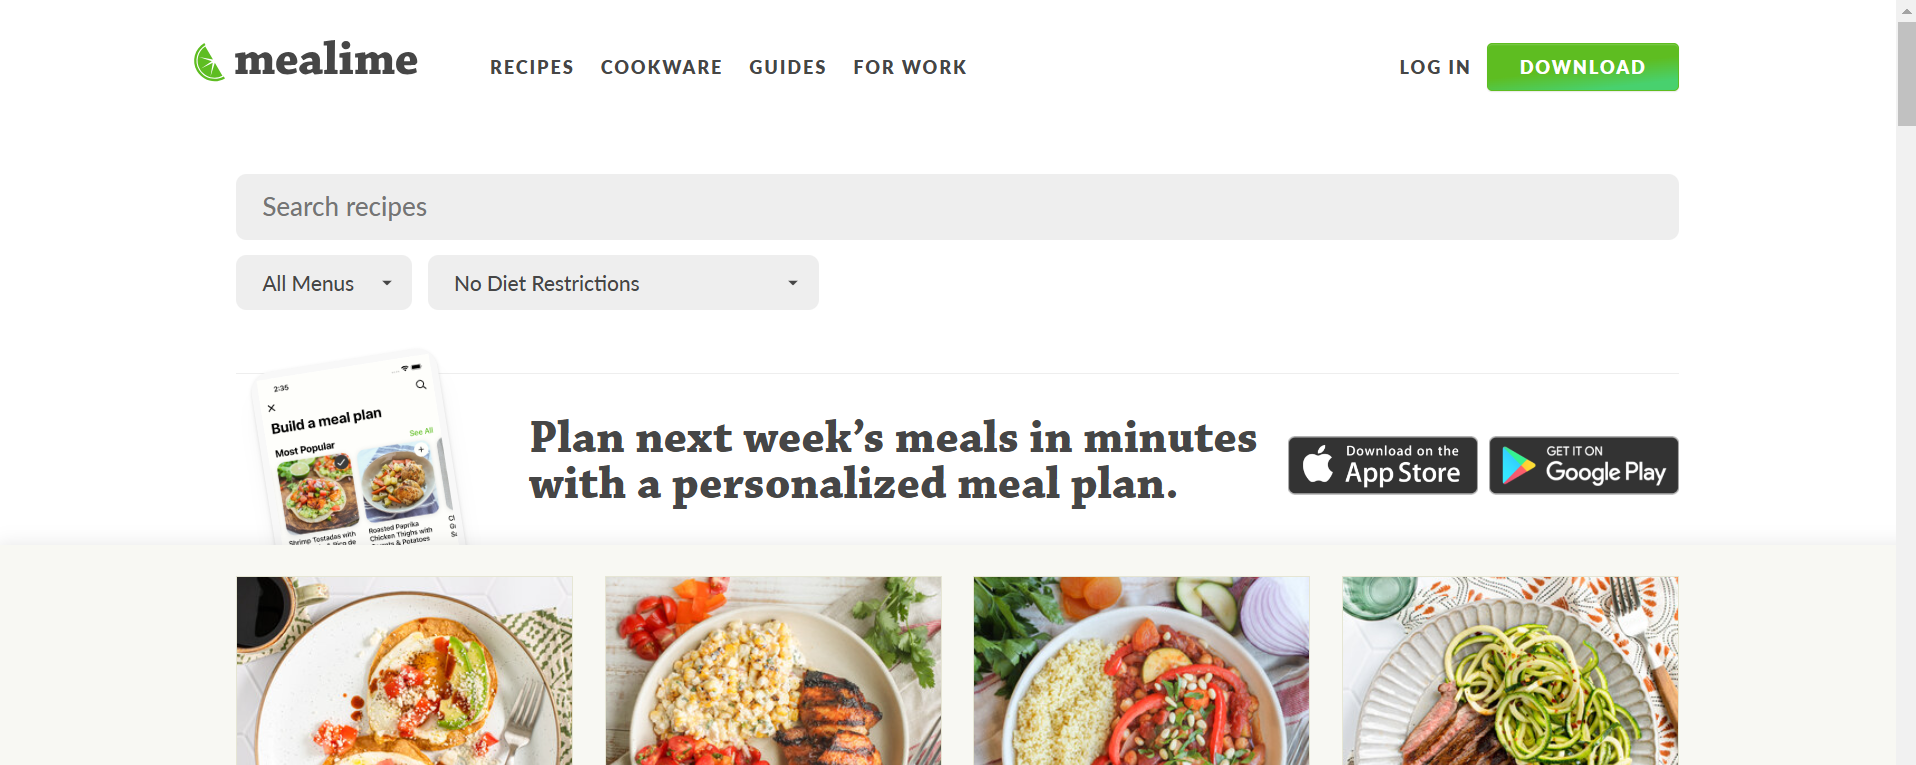
\includegraphics[width=0.9\textwidth]{mealime.png}
    

    \item \textbf{Meal planner grocery list} : Aplikace má kalendář s plánem menu, nákupním seznamem a seznamem s potravinami doma.
    \begin{itemize}
        \item Výhoda : Schopnost vytvářet pravidla jako „Pondělí je kuřecí den“.Schopnost vytvářet vlastní recepty a přidat zdrojové odkazy.
        \item Nevyhoda : Nedostatek automatizace při vytváření nákupního seznamu (po naplánování jídla je nutné přidat produkt do nákupního seznamu). Chybí možnost plánování jídla mimo domov.  Aplikace neposkytuje možnost sledovat datum expirace produktů
    \end{itemize}
    \begin{center}
         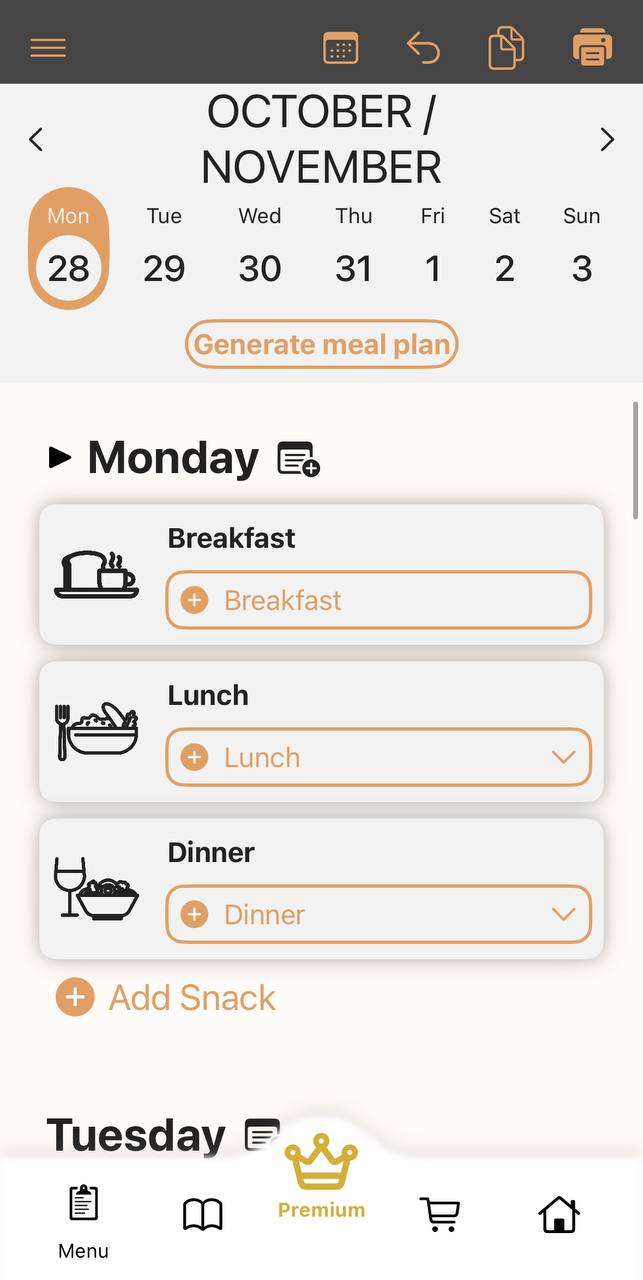
\includegraphics[width=0.35\textwidth]{grocerylist.png} % Шлях до зображення
    \end{center}
    
    \item \textbf{Daily Meal planner}
    \begin{itemize}
        \item Výhoda: V programu lze rozdělit přidané pokrmy na snídani, oběd a večeři. K dispozici je statistika spotřebovaných pokrmů za období, například posledních 30 dnů. Pokrmy jsou rozděleny do kategorií, z nichž každá je označena vlastní barvou, která se zobrazuje u pokrmu v kalendáři. K pokrmům lze přidat odkaz na web s receptem.
        \item Nevyhoda: Seznam produktů se nevyplňuje automaticky - uživatel musí vše zadávat ručně. Není také možné vést seznam produktů, které má uživatel k dispozici. Při zaplnění dne kalendáře pokrmy lze vytvořit nový pokrm a přidat ho do vybraného dne, například na snídani, ale nelze přidat žádné další informace kromě názvu pokrmu.
    \end{itemize}
   \begin{center}
        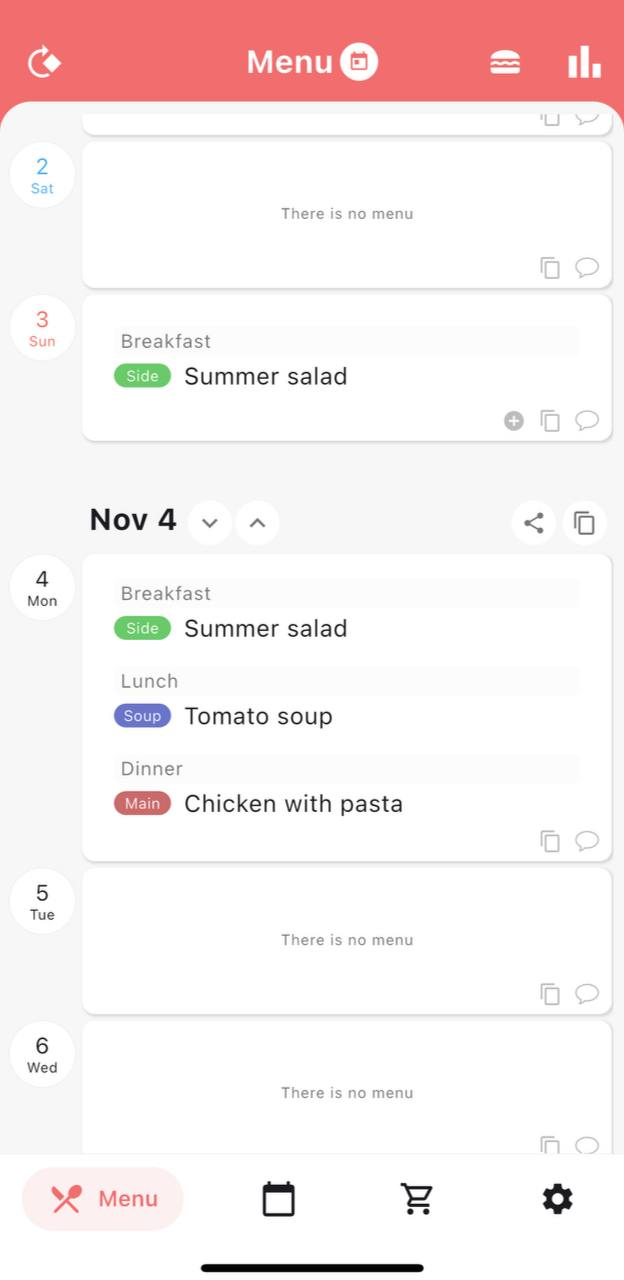
\includegraphics[width=0.3\textwidth]{Meal.jpg}
    \end{center}
    \item \textbf{Eatwell101}
    \begin{itemize}
        \item Výhoda: Program již obsahuje databázi s více než 3000 pokrmy, u nichž jsou uvedeny ingredience, recept, kalorická hodnota a další užitečné informace. Při přidání pokrmu do kalendáře se potřebné ingredience automaticky přidávají do seznamu produktů. Kromě přidání pokrmu do kalendáře je také možné uložit oblíbené pokrmy do vlastních receptů.
        \item Nevyhoda: Kalendář je určen pouze na týden, bez specifikace dnešního data. Není možné vytvářet vlastní recepty.
    \end{itemize}
    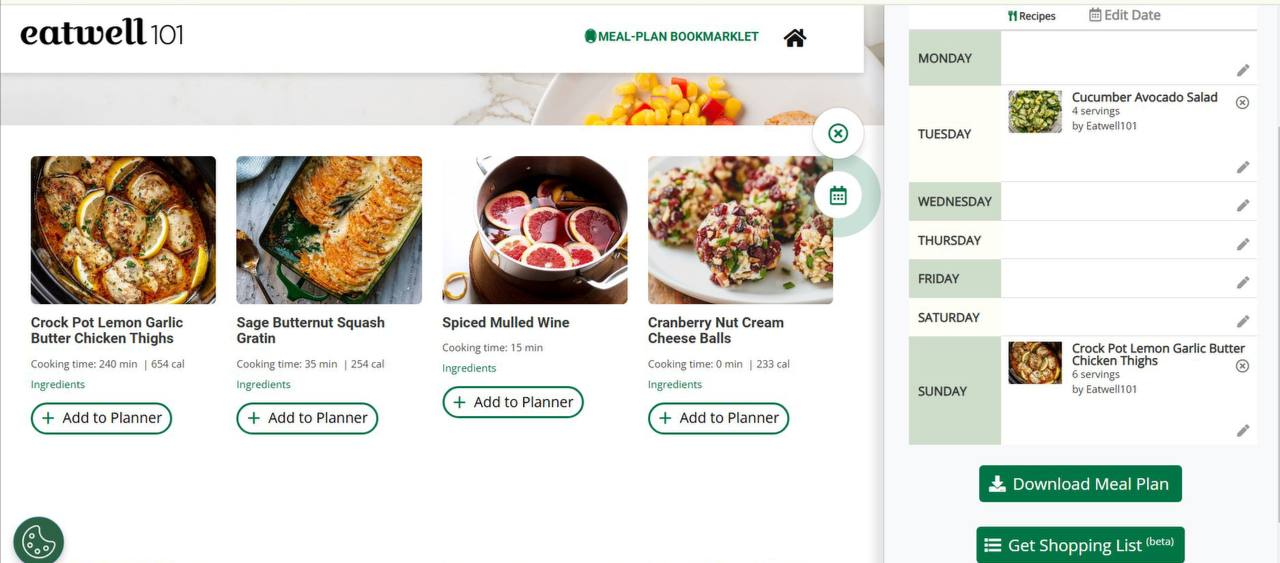
\includegraphics[width=0.9\textwidth]{eatwell101.jpg}
    
\end{itemize}


\subsection*{Závěry průzkumu}
\begin{itemize}
    \item Hlavním problémem studovaných aplikací je, že neumožňují kompletní plánování jídla. Některé aplikace pomáhají plánovat jídla podle data, ale nevytvářejí nákupní seznam, některé naopak. Chceme uživateli pomoci zautomatizovat celý proces plánování jídla: od nápadu na jídlo až po kalkulaci výdajů za měsíc. Líbil se nám nápad vytvořit si vlastní recepty. Také jsme se rozhodli rozdělit den na uživatelsky zvolený počet jídel pro usnadnění vizuálního plánování.
\end{itemize}


\section*{Návrh}
\subsection*{Návrh GUI}
 Rozdělili jsme naši aplikaci na nezávislé komponenty : Kalendář, ProductList, ShoppingList a DishesList. Horní menu pomáhá uživateli s navigací mezi sekcemi na webu.

 Calendar - tato komponenta představuje hlavní účel aplikace: jídelní plán.  Zobrazí se kalendář na měsíc, je možné si vybrat konkrétní den a naplánovat jídlo.
\begin{center}

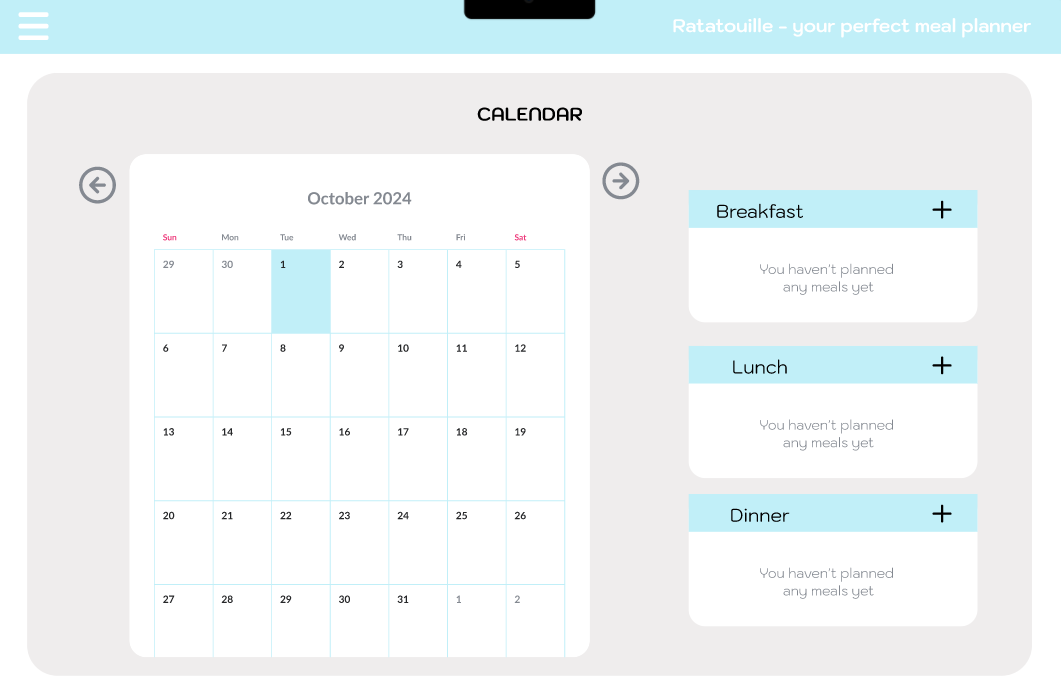
\includegraphics[width=0.7\textwidth]{figma_calendar.png}
\end{center}
ProductList – Tato komponenta zobrazuje seznam dostupných produktů a jejich krátký popis, které jsou připojeny k backendu a jsou přijímány prostřednictvím API požadavku. Díky Reactu lze seznam rychle aktualizovat bez nutnosti obnovovat celou stránku. Zobrazí se počet produktů, které se vejdou na obrazovku, je možné rolováním zobrazit další položky. Každý produkt lze snadno upravit nebo smazat.
\begin{center}
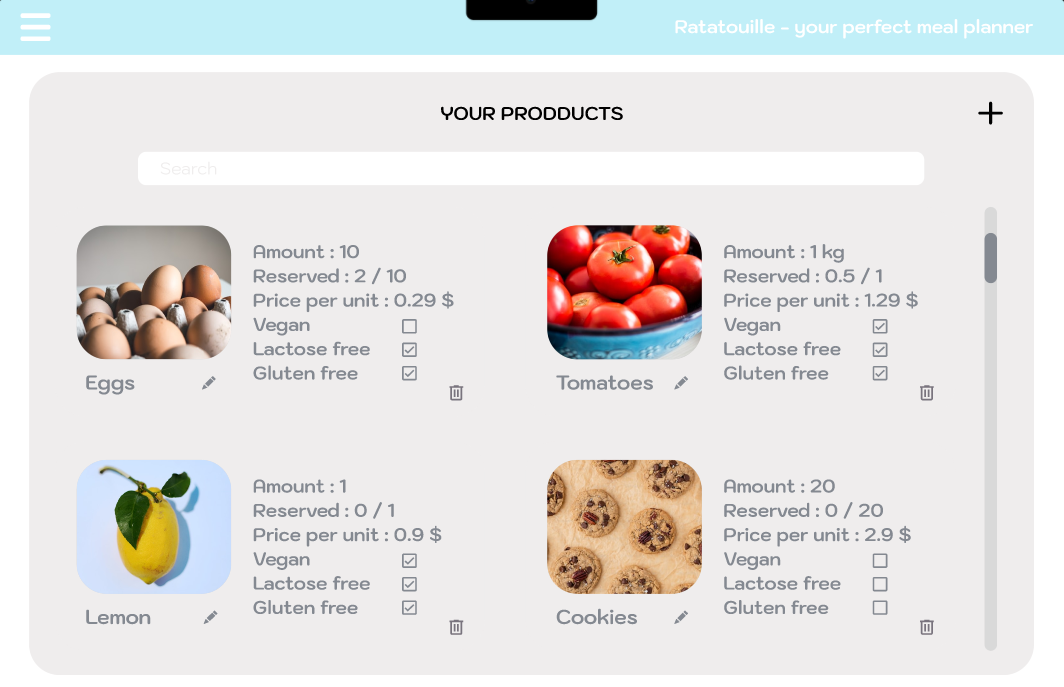
\includegraphics[width=0.7\textwidth]{figma_product.png}
\end{center}
\begin{center}
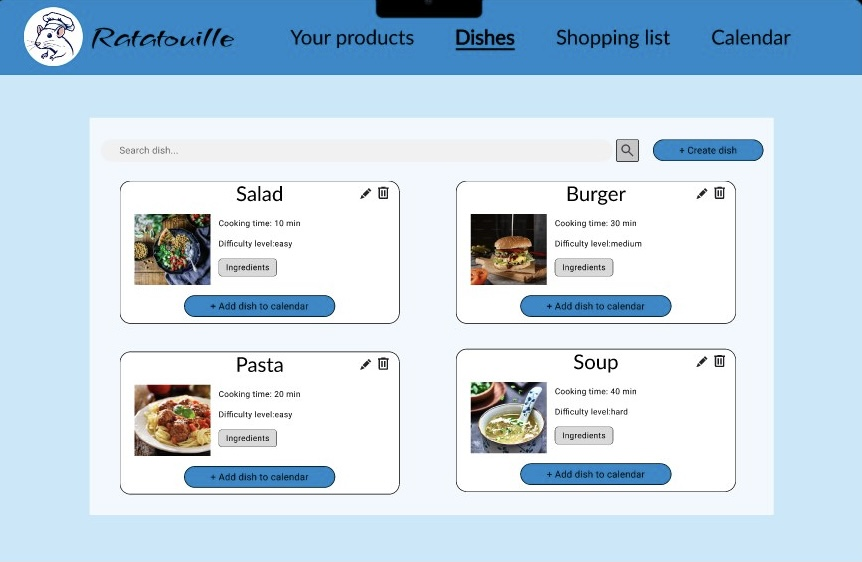
\includegraphics[width=0.9\textwidth]{dishes.JPG}
\end{center}
\begin{itemize}
    \item \textbf{Sekce Dish}: V této sekci se zobrazují jídla, která uživatel již vytvořil. Kromě možnosti vytvořit nové jídlo nebo vyhledat již existující, lze jídlo přidat do kalendáře na konkrétní datum. K dispozici jsou také základní funkce - úprava a smazání, které se zobrazují v pravém horním rohu každého jídla.
\end{itemize}
\begin{center}
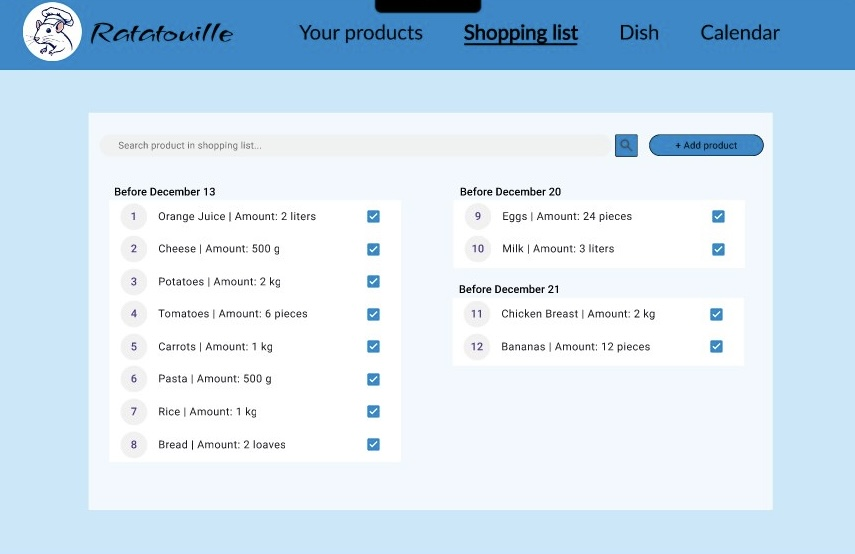
\includegraphics[width=0.9\textwidth]{shopping_list.JPG}
\end{center}
\begin{itemize}
    \item \textbf{Sekce Shopping List}: Produkty, které je třeba koupit, se zobrazují ve formě seznamu. Pokud je seznam příliš dlouhý, je k dispozici vyhledávací řádek pro snadnější navigaci. Pro přidání produktu se používá tlačítko v pravém horním rohu, pro odstranění se označí zaškrtávací políčko.
\end{itemize}
\subsection*{Výběr technologií}
\begin{itemize}
    \item Pro frontend jsme zvolili React, protože je to jeden z nejoblíbenějších frameworků pro vývoj dynamických a interaktivních uživatelských rozhraní. 
React také poskytuje pohodlnou architekturu komponent, která usnadňuje vytváření, opětovné použití a údržbu jednotlivých prvků rozhraní. Pro backend jsme zvolili Node.js ve spojení s frameworkem Express. Tato volba je odůvodněna snadným nastavením API, podobností s frontendem (používáme JavaScript na obou stranách) a integrací s databází MySQL.
\end{itemize}

\subsection*{Návrh API k BE}
\begin{itemize}
    \item Dish
    \begin{itemize}
        \item add$_$dish - přidá nové jídlo do tabulky Dishes, ve FE je pro to příslušné tlačítko, při jehož stisknutí se objeví formulář.
        \item get$_$dish - vyhledá potřebné jídlo v tabulce a vrátí všechny údaje o něm,  používá se při vyhledávání jídla.
        \item get$_$all - vrátí informace o všech jídlech, zobrazuje všechna jídla v sekci.
        \item change$_$dish - upraví informace o jídle
        \item delete$_$dish - odstraní jídlo z databáze, pro úpravu a odstranění jsou také k dispozici příslušná tlačítka.
        \item use$_$dish - vyhledá potřebné jídlo a ověří dostupnost produktů, které jsou k němu zapotřebí.
     \end{itemize}   
        
    \item Shopping List
     \begin{itemize}   
        
        \item add$_$list$_$product, delete$_$list$_$product, change$_$list$_$product, get$_$list$_$product, get$_$listAll$_$product- Podobně jako u podobných funkcí pro jídla, ale nyní pro tabulku Shopping list. Pro odstranění musí uživatel kliknout na zaškrtávací políčko vedle produktu, ostatní funkce jsou uživateli intuitivně zobrazeny.
     \end{itemize}   
        \item Product:
\begin{itemize}
    \item get product - vrací informace o produktu.
    \item get all products - vrací informace o produktech.
    \item add product - přidá produkt do databáze. Tlačítko + ve frontendu.
    \item delete product - odstraní produkt z databáze. Tlačítko odstranění ve frontendu.
    \item change product - změní atributy produktu. Tlačítko opravy ve frontendu.
    \item move to list - odebere produkt ze stávajících a přidá jej do seznamu produktů.
    \item check amount - zkontroluje množství produktu.
\end{itemize}

\item Calendar: 
\begin{itemize}
    \item get meal - vrátí informace o naplánovaném jídle. 
    \item add meal - přidá naplánovaném jídlo do databáze. Tlačítko + ve frontendu.
    \item delete meal - odstraní naplánované jídlo z databáze. Tlačítko odstranění ve frontendu.


    \end{itemize}
    \item  Klíčové datové struktury modelu:
    \begin{itemize}
    \item Dishes: tabulka, ve které jsou uloženy všechny informace o jídlech. Spojení M:N
s tabulkou Products, v tabulce spojení je navíc atribut, který uchovává množství produktu potřebné pro toto konkrétní jídlo.
\item Shopping List: tabulka, ve které jsou uloženy produkty, které si uživatel musí koupit.
\item Products: tabulka pro uchovávání produktů, které má uživatel k dispozici.
\item Calendar: tabulka dnů, do kterých uživatel přidal jídla. Má vztah M:N
s tabulkou Jídla, tabulka spojení obsahuje atribut, který určuje, zda je jídlo přidáno k snídani, obědu nebo večeři.
    \end{itemize}
\end{itemize}

\end{document}
